\chapter{IMPatienT : outil d’annotation et d’exploration de données multimodales de patients}

\section{Contexte}
Les données générées par la biopsie musculaire (imagerie et comptes-rendus textuels) sont non-structurées et nécessitent d'être annotées pour être utilisées par les algorithmes classiques de \gls{ml} afin d'en extraire de l'information. Dans ce contexte là, nous avons créé \gls{impatient} (fig. \ref{fig:impatient_logo}), une plateforme web permettant de numériser, d'annoter et d'explorer les données de biopsie musculaire. Développé en 2020-2021, c'est à dire avant la mise à disposition des \gls{llms}, \gls{impatient} repose sur le concept de vocabulaire standard (similaire à une ontologie) à définir par l'utilisateur, qui est la base permettant l'annotation des données.

\begin{figure}[htbp]
  \centering
  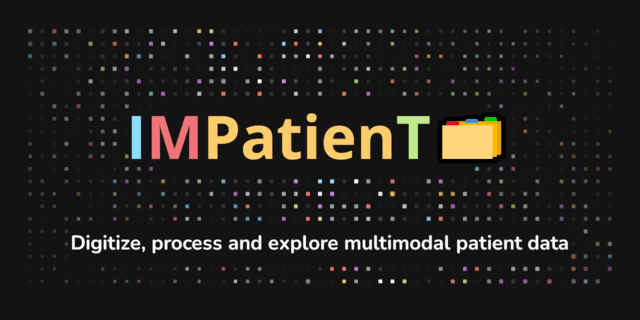
\includegraphics[width=0.7\textwidth]{figures/impatient_banner.png}
  \caption[Logo IMPatienT]{Logo de IMPatienT}
  \label{fig:impatient_logo}
\end{figure}


\section{Manuscrit} 
L'outil \gls{impatient} a fait l'objet de la rédaction d'un article qui a été soumis dans une revue scientifique à comité de lecture. Le manuscrit est présenté ci-dessous.

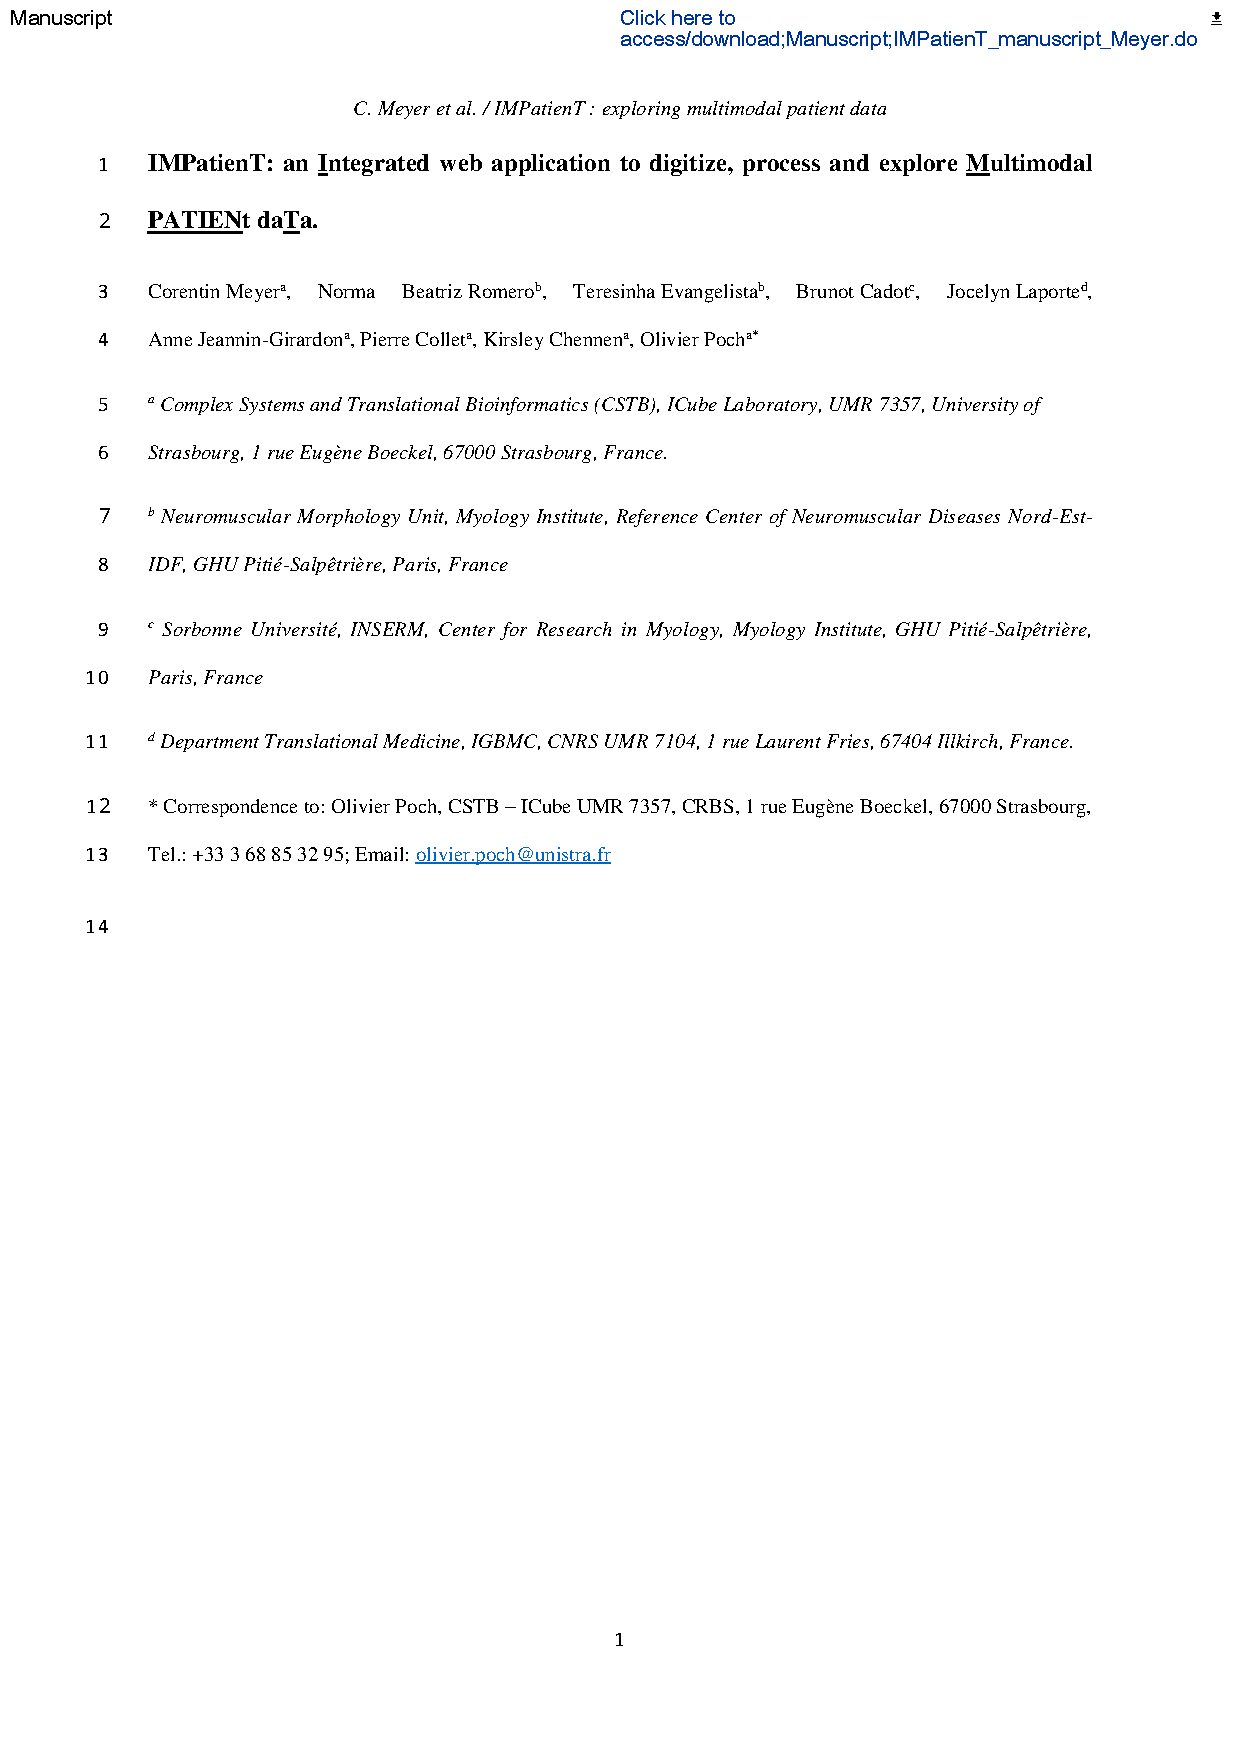
\includepdf[pages={1-27},scale=1,dpi=300]{corps/IMPatienT_pdf.pdf}
\section{Déploiement de la plateforme}
Afin de traiter les données de patients atteints de \gls{mc} (qui doivent restée privées) mais aussi de pouvoir faire une démonstration technique de l'outil, nous avons mis en ligne deux instances de la plateforme. Une première instance publique, à l'adresse \href{https://impatient.lbgi.fr}{https://impatient.lbgi.fr}, contient une quarantaine de rapports de comptes rendus fictifs générés aléatoirement. Cette instance est accessible à tout le monde et est remise à zéro chaque jours. Une seconde instance privée, à l'adresse \href{https://myoxia.lbgi.fr}{https://myoxia.lbgi.fr}, contient 89 rapports de comptes rendus de patients réels provenant de l'Institut de Myologie de Paris qui ont été numérisés. Cette instance n'est accessible que par mot de passe et son contenu est sauvegardé de façon journalière. Le code-source d'\gls{impatient} est \textit{open-source} et disponible dans un répertoire GitHub à l'adresse: \href{https://github.com/lambda-science/IMPatienT}{https://github.com/lambda-science/IMPatienT}
\section{Limitations}
\gls{impatient} est une plateforme permettant d'annoter et d'explorer les données biomédicales issues de la biopsie musculaire de patients atteints de \gls{mc}. Cependant l'approche utilisée pour l'annotation est semi-automatique et requiert donc toujours un travail manuel et humain d'annotation. Cette limitation empêche donc le passage à l'échelle et le traitement d'une masse importante de comptes rendus textuels ou d'images. De plus l'approche utilisée est dépendante de la définition d'un vocabulaire standard exhaustif. Si un terme nouveau est présent dans un compte-rendu et est absent du vocabulaire au moment de l'annotation, il faut le rajouter au préalable. De même, si on opère des modifications importantes du vocabulaire standard, il est peut être nécessaire de devoir passer en revu l'ensemble des comptes-rendus déjà numérisés pour vérifier si des nouveaux termes sont à associer aux compte-rendus ou d'anciennes annotations à supprimer.
\section{Perspectives de développement}
En terme développement futur, il est nécessaire d'intégrer à \gls{impatient}  de nouveaux outils permettant l'automatisation de l'analyse des compte-rendus, comme par exemple un outil permettant de pré-remplir les formulaires avec les informations générales détectées. Mais aussi de proposer des alternatives plus automatiques au système d'annotation avec le vocabulaire standard. C'est l'objet de l'outil \gls{nlmyo} présenté dans un prochain chapitre.

De plus au niveau de l'analyse d'images, il est intéressant de proposer un outil capable de quantifier automatiquement sur base d'algorithmes et d'\gls{ia} des marqueurs pathologiques dans les images de biopsie, car cette information est manquante dans les compte-rendus de biopsie, les observations ne sont que qualitatives. C'est aussi l'objet d'un outil présenté dans un prochain chapitre nommé \gls{myoquant}.

Grâce à l'intégration de ces outils, l'application \gls{impatient} deviendrait le socle de l'intégration de plusieurs outils d'\gls{ia} pour l'analyse de données multimodales. \gls{impatient} serait alors le point d'entrée mettant à disposition des outils pour créer une base de données multimodales de patients et fournir les outils adaptés à leur analyse et exploration.